\documentclass[conference]{IEEEtran}
\IEEEoverridecommandlockouts
% The preceding line is only needed to identify funding in the first footnote. If that is unneeded, please comment it out.
\usepackage{cite}
\usepackage{amsmath,amssymb,amsfonts}
\usepackage{algorithmic}
\usepackage{graphicx}
\usepackage{textcomp}
\usepackage{xcolor}
\def\BibTeX{{\rm B\kern-.05em{\sc i\kern-.025em b}\kern-.08em
    T\kern-.1667em\lower.7ex\hbox{E}\kern-.125emX}}
\begin{document}

\title{Context Aware Empathetic Text Generation for Mental Health Support
% {\footnotesize \textsuperscript{*}Note: Sub-titles are not captured in Xplore and
% should not be used}
% \thanks{Identify applicable funding agency here. If none, delete this.}
}

\author{\IEEEauthorblockN{1\textsuperscript{st} Given Name Surname}
\IEEEauthorblockA{\textit{dept. name of organization (of Aff.)} \\
\textit{name of organization (of Aff.)}\\
City, Country \\
email address or ORCID}
\and
\IEEEauthorblockN{2\textsuperscript{nd} Given Name Surname}
\IEEEauthorblockA{\textit{dept. name of organization (of Aff.)} \\
\textit{name of organization (of Aff.)}\\
City, Country \\
email address or ORCID}
\and
\IEEEauthorblockN{3\textsuperscript{rd} Given Name Surname}
\IEEEauthorblockA{\textit{dept. name of organization (of Aff.)} \\
\textit{name of organization (of Aff.)}\\
City, Country \\
email address or ORCID}
\and
\IEEEauthorblockN{4\textsuperscript{th} Given Name Surname}
\IEEEauthorblockA{\textit{dept. name of organization (of Aff.)} \\
\textit{name of organization (of Aff.)}\\
City, Country \\
email address or ORCID}
\and
\IEEEauthorblockN{5\textsuperscript{th} Given Name Surname}
\IEEEauthorblockA{\textit{dept. name of organization (of Aff.)} \\
\textit{name of organization (of Aff.)}\\
City, Country \\
email address or ORCID}
\and
\IEEEauthorblockN{6\textsuperscript{th} Given Name Surname}
\IEEEauthorblockA{\textit{dept. name of organization (of Aff.)} \\
\textit{name of organization (of Aff.)}\\
City, Country \\
email address or ORCID}
}

\maketitle

\begin{abstract}
Emotional distress such as depression and anxiety affects a large part of the global population, yet financial cost, social stigma and a shortage of mental health specialists keep many people from care. Advances in Natural Language Processing (NLP) have made dialogue support systems possible, and conversational agents are now widely used as a supplement to mental health support. Many systems built on Large Language Models (LLMs), however, respond in an emotionally generic and contextually indifferent way, and the emotional judgement behind a reply is never recorded, which limits their value in mental health care. This paper investigates the production of contextually thoughtful and emotionally responsive text on a single consumer graphics card. A RoBERTa-base emotion detector, fine-tuned on the first message of each EmpatheticDialogues conversation, passes its three most probable of 32 emotions and the words its attention selected to a 4-bit Phi-4-mini generator, which first chooses one emotion and then writes the reply under guidance written for that emotion. Twelve systems answer the same 300 test conversations and are compared on rule adherence, an independent empathy classifier, emotional fidelity, a blind panel of two LLM judges and a study with 40 human raters, using paired tests corrected for multiple comparisons. The detector reaches 50.3\% top-1 and 84.3\% top-5 accuracy. The decoupled system expresses the person's true emotion more often than any other system, is more empathetic than a single model of its own size and than its own generator used alone, and runs in 3.40 GB of memory with 52\% of the parameters of a 7.6-billion-parameter single model. Human raters scored it highest on empathy, relevance and supportiveness and preferred its replies in 61.3\% of 320 blind choices. The research focuses on support and the absence of diagnosis.
\end{abstract}

\begin{IEEEkeywords}
Empathetic text generation, natural language processing, emotion-aware language modeling, computational empathy, contextual dialogue modeling, emotionally intelligent LLM
\end{IEEEkeywords}

\section{Introduction}
People increasingly bring their difficulties to a screen. A student who cannot sleep before an examination, who has just lost a pet, or who has moved to a new city and spoken to nobody for weeks is more likely to type the sentence than to say it aloud. The number of people who need mental health services far exceeds the services available \cite{b1}, and text-based support has become the step between having nobody to tell and seeing a professional. Here a reply that is factually helpful but emotionally wrong does not merely fail to help. Empathy in such support can be made concrete: the EPITOME framework divides a supportive reply into emotional reactions, interpretations and explorations \cite{b2}, while counselling guidance warns that a series of questions turns support into an interrogation \cite{b3}.

Two families of systems attempt this task, and both hide the decision that matters most. Joint models trained on EmpatheticDialogues learn the emotion inside the network as an auxiliary objective of generation \cite{b4,b5,b6,b7,b8,b9,b10}, and four years of architectural work have raised their emotion accuracy only from 30.6\% to 41.2\%. The newer approach hands the whole task to a large language model (LLM) steered by prompting, tools, personality signals or step-by-step emotional reasoning \cite{b11,b12,b13,b14,b15}. People prefer these replies, but the model's emotional judgement is no more reliable than a small purpose-trained classifier's \cite{b16,b17}, and it is never recorded.

Four problems follow, and they compound. \textit{Nothing can be inspected:} no emotion is recorded, so nobody can check it and no safeguard can sit between reading the message and writing the reply. \textit{Quality is tied to hardware:} the strongest results need models too large for the equipment a university well-being service or a small charity owns, so using them sends what a distressed person typed to another organisation's computer. \textit{The measures reward the wrong thing:} overlap with one reference reply rewards resemblance to the corpus and is blind to the characteristic weakness of machine empathy, kind replies drawn repeatedly from the same few phrases \cite{b18}. \textit{Comparisons do not separate the design from the generator:} where a separated design beats a single model the generator has usually changed too, and the one framework with a comparable two-stage structure builds it as an internal reasoning step and does not test it under a memory limit \cite{b19}.

This paper therefore asks: \textit{does detecting the emotion in a separate, visible step produce better empathetic replies than asking one model to do both, when the whole system must fit on a single consumer GPU?} Our contributions are:
\begin{itemize}
\item A decoupled pipeline running in 3.40 GB on an 8 GB GPU, in which a RoBERTa-base detector passes its top-3 emotions and attention-derived cue words to a 4-bit Phi-4-mini generator that chooses one emotion before writing under guidance specific to it, so every reply carries a record of the feeling it answered.
\item A controlled comparison of twelve systems on the same 300 conversations, including the system's own generator used alone, separating the effect of the design from that of generator size.
\item A five-signal evaluation: rule adherence, an empathy classifier trained on human ratings, emotional fidelity, a blind two-judge LLM panel and a study with 40 human raters, with paired tests and Holm correction.
\item Evidence that detection accuracy does not limit reply quality, and two negative results, for retrieval augmentation and fine-tuning, traced to one measured property of the corpus.
\end{itemize}

\section{Related Work}\label{sec:related}

\subsection{The Benchmark and Joint Models}
EmpatheticDialogues (ED) \cite{b20,b21} pairs a speaker describing a situation tied to one of 32 fine-grained emotions with a listener's reply. The granularity forces a system to separate feelings such as \textit{sad}, \textit{lonely}, \textit{disappointed} and \textit{devastated}. Its fastText classifier reached about 43\%, but on the situation description, written after the fact and naming the feeling more explicitly than a speaker's own message. Joint models then added mechanisms to one encoder-decoder trained from scratch: emotion-specific listeners \cite{b4}, emotion mimicry \cite{b5}, an adversarial discriminator \cite{b6}, commonsense knowledge \cite{b7,b8}, cognition-affection alignment \cite{b9} and emotion-semantic vectors \cite{b10}. RoBERTa-GPT2, built from pre-trained components instead, reaches 51.5\% on the same task \cite{b22}: on a corpus this size the limit is how little text a model has seen, not what is built into it. On the listener side, supportive replies in ED draw on a small, describable set of intents such as acknowledging and questioning \cite{b23}.

\subsection{Large Language Models and Emotion}
Human raters strongly prefer ChatGPT to purpose-built models (4.64 against 3.08 out of 5 for CEM), and replies improve when the emotion is supplied explicitly \cite{b11,b12}. Each later source of structure carries a cost: tool calling needs a fine-tuned 7B model on 48 GB GPUs \cite{b13}, personality conditioning needs visual input and reaches 45.4\% from text \cite{b14}, competitive emotional-support systems fine-tune models up to 72B parameters \cite{b24}, and emotion-aware retrieval reports gains short of significance with no human evaluation \cite{b25}. A systematic review finds LLM replies often rated as empathetic as clinicians', with sameness as their weakness \cite{b18}.

Recognition is a separate question. Emotion in conversation depends on context \cite{b26} and is often implied \cite{b27}; LLMs are no better at recognising it than purpose-trained classifiers \cite{b16}, and fine-tuned small encoders beat zero-shot LLMs on multi-label emotion by about 72 to 46 \cite{b17}. A deployed agent's RoBERTa classifier reported about 61.5\% on the first ED utterance \cite{b28}, a validation-set score from a technical report rather than a held-out result. The same machinery serves clinical screening \cite{b29,b30}, where scarce data and bias remain open \cite{b31}.

\subsection{The Closest Prior Work and Evaluation}
The Hybrid Empathetic Framework adds a small empathetic model to an LLM and predicts the emotion in two steps \cite{b19}. That is the same architectural intuition, and we claim no priority for it. It targets benchmark performance; ours runs within 8 GB so a disclosure never leaves the machine, keeps the emotional decision as a record on every reply, and is judged by what a supportive reply must do. Our contribution is what the separation provides and the controlled evidence for it. For evaluation, strong LLM judges agree with human preference over 80\% of the time but favour longer answers \cite{b32} and their own family \cite{b33}, so panels from different developers are preferred \cite{b34}; the WASSA 2024 shared task provides empathy classifiers trained on human ratings \cite{b35,b36}; and human evaluation, as ratings \cite{b11} or preferences \cite{b13}, remains the reference.

\section{Methodology}\label{sec:method}

\subsection{Data and Preparation}
All data come from ED \cite{b20}: 23,144 conversations and 88,687 utterances, each conversation labelled with one of 32 emotions. The project began on GoEmotions \cite{b37} and abandoned it for four measured reasons: its comments carry no replies; \textit{neutral} is its largest class at 32.75\%; the states support must answer are its rarest, with \textit{grief} appearing 96 times against 5,122 for \textit{admiration}; and 16.25\% of examples carry several labels. In ED the literal string \texttt{\_comma\_} was restored, unparsable rows discarded and empty utterances removed. Only the first user message of each conversation is kept, because that is what the system receives when someone starts typing. This was the most consequential decision of the project: a GPT-2 detector trained on situation descriptions scored 56.9\% on situation text but 48.2\% on real first messages. Inputs are capped at 128 tokens, covering 99.7\% of first messages, with no lower-casing, stemming or stop-word removal, since capitalisation and words such as \textit{not} carry feeling. The official split gives 17,839 training, 2,763 validation and 2,542 test conversations. Every generation experiment uses the same 300 test conversations (seed 42); 64 of them, the shortest and longest per emotion, go to the AI judges, and 8 to the human study.

\subsection{Response Rules}
Every reply must (R1) acknowledge the feeling, (R2) ask exactly one question and (R3) stay within 120 words. R1 follows EPITOME's emotional reactions \cite{b2}; R2 avoids both a reply with no invitation to continue and the question-and-answer trap \cite{b3}; R3 is our own readability requirement. Within systems, replies with an acknowledgement score 0.36 points higher on the empathy classifier ($p<0.001$, 3,300 replies) and replies within the limit score 0.65 points higher on judged empathy ($p=0.006$); no measure rewards R2, which we keep as a usability and safety requirement. The rules cannot be met by imitating the corpus: only 4.3\% of ED listener replies satisfy all three.

\subsection{Emotion Detector}
Five detectors were trained with one script and seed, changing only the backbone: GPT-2 Medium (355M), BERT-base \cite{b38}, ELECTRA-base, RoBERTa-base \cite{b39} (125M) and RoBERTa-large, each a transformer \cite{b40} with a 32-way head and cross-entropy loss. Settings were learning rate $2\times10^{-5}$, effective batch 16, at most four epochs with early stopping on validation accuracy, 6\% linear warm-up, weight decay 0.01 and 16-bit mixed precision. Base-size encoders were indistinguishable on top-1 accuracy (48.8--50.2\%) and separated only on ranking quality, where RoBERTa-base led; since the design consumes a ranking, it was selected. RoBERTa-large added 2.9 points of top-1 accuracy at 2.8 times the parameters and 7.4 times the training time.

\subsection{Attention-Derived Cue Words}
So that the reply can refer to what the person wrote, the detector reports the words it attended to. With final-layer attention $A\in\mathbb{R}^{H\times T\times T}$ over $H$ heads and $T$ tokens, the cue score of token $t$ is the attention paid to it by the classification token, averaged over heads:
\begin{equation}
s(t)=\frac{1}{H}\sum_{h=1}^{H}A_{h,0,t}.\label{eq:cue}
\end{equation}
Sub-word scores from \eqref{eq:cue} are summed into words, special tokens are dropped, and the top 40\% of words are kept (at least three, at most fourteen). The attention implementation must be requested explicitly, because the library default returns no weights and raises no error; the system checks this at start-up and stops if weights are missing.

\subsection{Two-Stage Generator}
The generator is Phi-4-mini-instruct \cite{b41} (3.8B) in 4-bit NF4 double quantisation \cite{b42}; the whole system has 3.96B parameters. With the detector, prompt, rules, data and decoding fixed, it followed all three rules in 65.3\% of replies against 57.7\% for Qwen2.5-1.5B \cite{b43} and 22.0\% for Gemma-3-4B \cite{b44}. Fig.~\ref{fig:pipeline} shows the pipeline. In \textit{stage 1} the generator sees the message and the three candidates and names the one that best fits, by greedy decoding capped at ten tokens, so the recorded choice is reproducible. In \textit{stage 2} the system prompt is assembled from the chosen emotion, the cue words, guidance written for that emotion (one of 32 blocks; for \textit{lonely}, acknowledge the isolation and offer no surface-level fix) and the three rules. Decoding uses temperature 0.7, top-p 0.9 \cite{b45}, at most 250 new tokens and seed 42, identical for every system compared. Every reply is stored with the candidates, their confidences, the chosen emotion and the cue words.

\begin{figure}[htbp]
\centerline{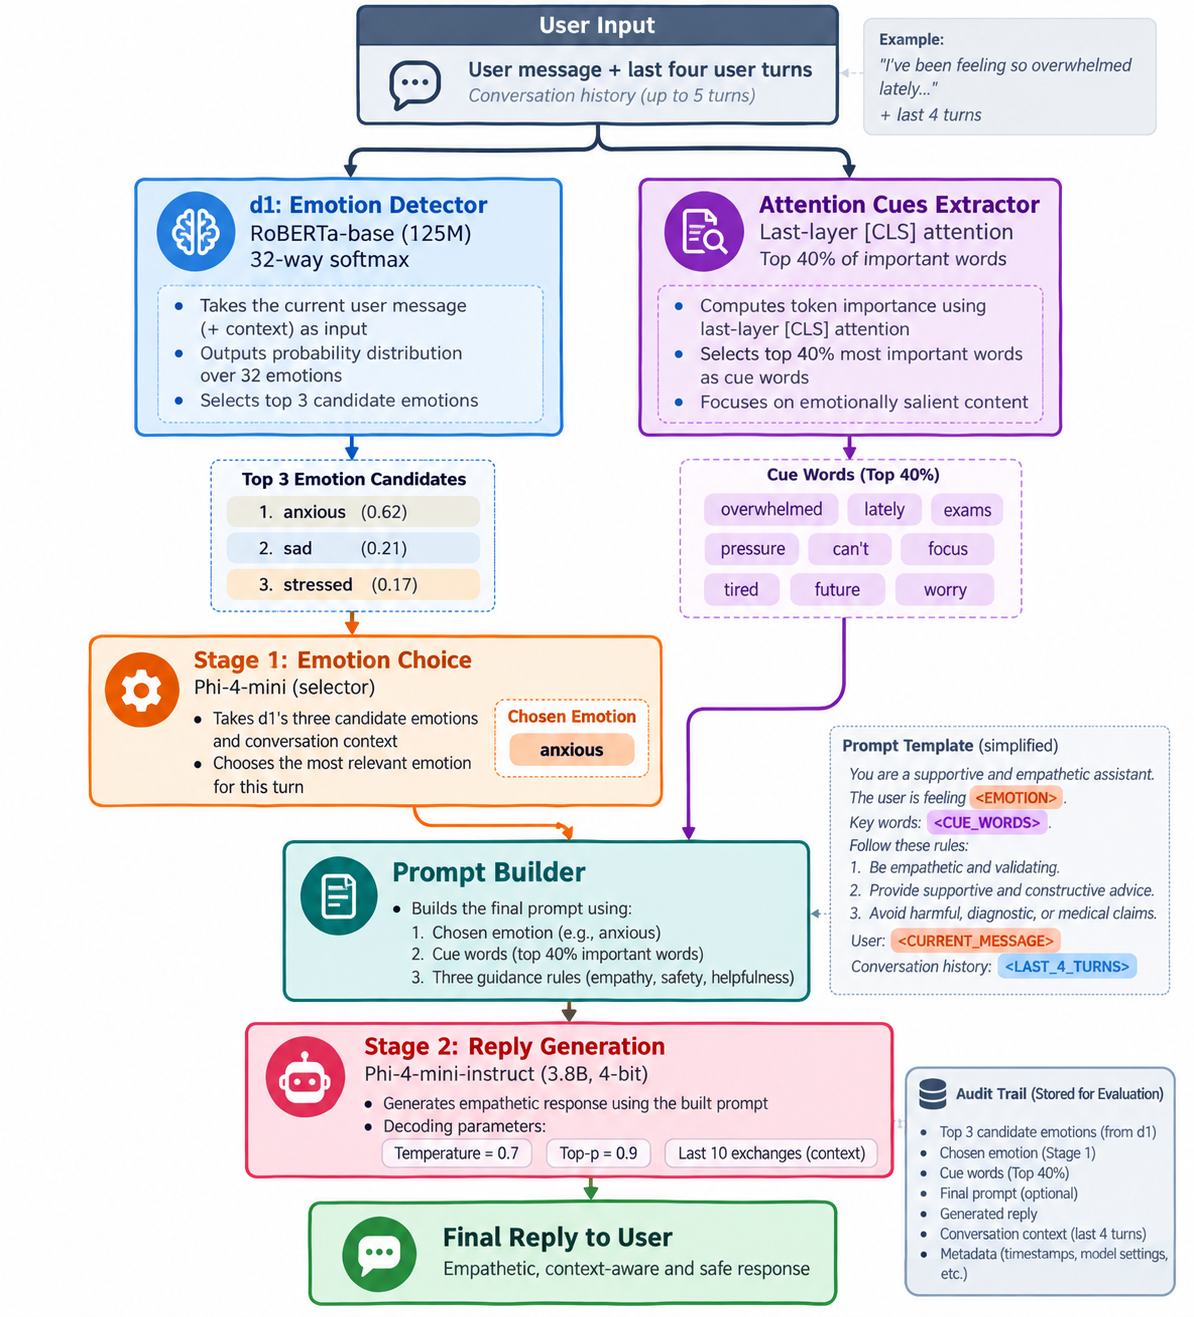
\includegraphics[width=0.92\columnwidth]{fig_pipeline.png}}
\caption{The complete two-stage pipeline of the proposed system.}
\label{fig:pipeline}
\end{figure}

The separate stage-1 call was chosen by measurement over four alternatives: the top label alone, the top label hedged when the detector is unsure, every emotion above probability 0.05, and the top three resolved inside the generation call. Several emotions in one prompt give contradictory guidance, and resolving the emotion in the same call as the reply damaged rule-following.

\subsection{Designs Without a Detector and the Agent}
Six designs reply without a detector. Three prompt a single model to identify the emotion silently and reply under the same rules, at 1.5B (Qwen2.5-1.5B), 7.6B (Qwen2.5-7B, 4-bit) and with our own 3.8B generator; the last is the proposed system with the detector removed. A zero-shot baseline is asked only to be caring; a fine-tuned baseline adapts Qwen2.5-1.5B with LoRA \cite{b46} (rank 16, alpha 32, learning rate $2\times10^{-4}$) on 17,749 message-reply pairs; and a retrieval-augmented variant \cite{b47} places the two most similar human replies, found with all-MiniLM-L6-v2 embeddings \cite{b48}, in the prompt.

The same pipeline runs once per turn as a conversational agent. The detector reads the user's last four turns; the generator keeps the last ten exchanges verbatim; from the second turn the question rule relaxes to at most one, because a question every turn is an interrogation; and when the detected emotion changes, the prompt names the shift.

\section{Experimental Setup}\label{sec:setup}
\textit{Rule adherence} is checked mechanically: a fixed list of 13 acknowledgement phrases, exactly one question mark, at most 120 words. The \textit{empathy classifier} is the WASSA 2024 hyy33 system \cite{b36}, trained on human empathy ratings of conversation turns and correlating with them at $r=0.544$ \cite{b35}, scoring 0 to 10. \textit{Emotional fidelity} applies the detector to the reply and asks whether the emotion it expresses matches the conversation's label. \textit{Repetition} is the share of a system's replies containing one of its own ten most frequent five-word phrases.

\textit{AI judges:} Nemotron 3 Ultra and gpt-oss-120b, from developers unrelated to our models \cite{b33}, score each reply blind from 1 to 10 for empathy, relevance and safety at temperature 0. Because judges span 3.9 to 8.2 and the classifier only 3.4 to 5.8, the three raters are standardised across the eight judged systems and averaged into a panel score; weighting the classifier at 50\% instead of 33\% leaves the ranking almost unchanged (rank agreement 0.98).

\textit{Human study:} 40 participants, mostly students, read 8 situations, each with replies from the proposed system and the same-size and larger single models in counterbalanced order without system names. They rated each reply from 1 to 5 for empathy, contextual relevance and supportiveness, then chose the best reply: 2,880 ratings and 320 choices. Participation was voluntary and anonymous, no personal details were collected, distressing content was flagged in advance and participants could stop at any time.

\textit{Statistics:} all comparisons are paired. Binary outcomes use McNemar's exact test \cite{b49} and scores the Wilcoxon signed-rank test \cite{b50}, each with a 95\% bootstrap interval from 10,000 resamples \cite{b51}; p-values are Holm-corrected \cite{b52} within each measure. A difference counts only when the corrected $p<0.05$ \textit{and} the interval excludes zero. Human ratings are tested on per-participant means. Experiments used PyTorch \cite{b53}, Transformers \cite{b54}, SciPy \cite{b55} and scikit-learn \cite{b56} on one NVIDIA RTX 4060 with 8 GB \cite{b57}.

\section{Results}\label{sec:results}

\subsection{Emotion Detection}
The deployed detector reaches 50.3\% top-1, 76.5\% top-3 and 84.3\% top-5 accuracy on all 2,542 test conversations, with macro-F1 of 49.4\% against a 3.1\% chance level; accuracy and weighted-F1 differ by 0.9 points, so the result is not driven by common emotions. The errors matter more than their number: all twelve of the most frequent confusions are near neighbours such as \textit{afraid}/\textit{terrified} and \textit{sad}/\textit{devastated}, which is why three candidates are passed on. Table~\ref{tab:published} shows the detector exceeding every published joint model and both of the dataset's own classifiers while reading only the first message. It starts from an encoder pre-trained on about 160 GB of text rather than GloVe vectors, does one job, and is trained on the text it receives; as those models were not re-trained under our setting, we do not claim the best detector on ED.

\begin{table}[htbp]
\caption{Emotion Recognition on EmpatheticDialogues}
\begin{center}
\begin{tabular}{|l|l|c|c|}
\hline
\textbf{System} & \textbf{Input} & \textbf{Top-1} & \textbf{Top-5} \\
\hline
EmpDG \cite{b6} & Joint, dialogue & 30.64 & -- \\
MoEL \cite{b4} & Joint, dialogue & 30.75 & -- \\
MIME \cite{b5} & Joint, dialogue & 31.21 & -- \\
KEMP \cite{b7} & Joint, dialogue & 36.57 & -- \\
CEM \cite{b8} & Joint, dialogue & 37.81 & -- \\
CASE \cite{b9} & Joint, dialogue & 38.92 & -- \\
ESCM \cite{b10} & Joint, dialogue & 41.19 & -- \\
Personality-aware \cite{b14} & Joint, text & 45.4 & -- \\
EmpSOA \cite{b14} & Joint, text & 48.3 & -- \\
fastText \cite{b20} & Situation & 43.0 & -- \\
DeepMoji \cite{b20} & Situation & 48.0 & -- \\
\hline
\textbf{Ours, RoBERTa-base} & \textbf{First msg.} & \textbf{50.3} & \textbf{84.3} \\
\hline
\end{tabular}
\label{tab:published}
\end{center}
\end{table}

\subsection{What the Replies Do}
Table~\ref{tab:main} gives the mechanically checked behaviour of all twelve systems. The proposed system follows all three rules in 60.0\% of replies, below the 7.6B single model (82.3\%) and its own generator alone (73.7\%) and above the same-size single model (51.3\%). It has the highest emotional fidelity of all twelve at 36.7\%, against 32.3\% for the largest single model and 27.0\% for its own generator alone. The fine-tuned model reproduces the corpus style, ten-word replies that rarely acknowledge the feeling, and Gemma-3-4B breaks the length limit in 72\% of replies. The detector's three candidates contain the gold emotion in 78.0\% of conversations, and the generator overrides the detector's first choice in 40.7\%. Repetition falls to 58.7\% from 72.3\% for the same generator alone.

\begin{table*}[htbp]
\caption{What Every Reply Does: Rule Checks, Length and Emotional Fidelity on 300 Test Conversations}
\begin{center}
\begin{tabular}{|l|c|c|c|c|c|c|}
\hline
\textbf{System} & \textbf{Ack. (\%)} & \textbf{One Q. (\%)} & \textbf{$\leq$120 w. (\%)} & \textbf{All rules (\%)} & \textbf{Words} & \textbf{Fidelity (\%)} \\
\hline
Single model Qwen2.5-7B & 83.0 & 99.0 & 100.0 & \textbf{82.3} & 53 & 32.3 \\
Single model Phi-4-mini (generator alone) & 77.3 & 96.0 & 99.3 & 73.7 & 73 & 27.0 \\
RoBERTa + Phi-4-mini, top-1 & 72.0 & 94.7 & 96.0 & 65.3 & 80 & 28.3 \\
Initial pipeline (GPT-2 + Qwen2.5-1.5B) & 70.3 & 87.3 & 100.0 & 63.7 & 35 & 26.0 \\
\textbf{Proposed: two-stage RoBERTa + Phi-4-mini} & 66.3 & 92.7 & 100.0 & 60.0 & 57 & \textbf{36.7} \\
RoBERTa + Qwen2.5-1.5B, top-1 & 67.7 & 84.3 & 100.0 & 57.7 & 35 & 25.3 \\
Single model Qwen2.5-1.5B & 70.7 & 73.7 & 100.0 & 51.3 & 42 & 25.7 \\
Initial pipeline + retrieval & 57.0 & 78.0 & 100.0 & 43.7 & 34 & 27.7 \\
Two-stage Qwen2.5-1.5B & 47.0 & 74.3 & 99.7 & 36.7 & 44 & 27.0 \\
Fine-tuned Qwen2.5-1.5B (LoRA) & 30.0 & 74.0 & 100.0 & 22.3 & 10 & 18.3 \\
RoBERTa + Gemma-3-4B, top-1 & 96.7 & 92.0 & 27.7 & 22.0 & 133 & 35.0 \\
Zero-shot Qwen2.5-1.5B & 81.7 & 22.7 & 83.7 & 19.0 & 76 & 24.7 \\
\hline
\end{tabular}
\label{tab:main}
\end{center}
\end{table*}

\subsection{The Empathy Panel}
In Table~\ref{tab:panel} the 7.6B single model leads (+1.11), followed by the proposed system (+0.59), first among systems that fit 8 GB. The judges agree reply by reply at Spearman $\rho=0.69$ and the classifier ranks the systems as they do ($\rho=0.74$). The four leading systems all use a generator of at least 3.8B parameters and do not differ significantly on the judges' scores after correction.

\begin{table}[htbp]
\caption{The Empathy Panel}
\begin{center}
\begin{tabular}{|l|c|c|c|c|}
\hline
\textbf{System} & \textbf{Nemo.} & \textbf{GPT-oss} & \textbf{WASSA} & \textbf{Panel} \\
\hline
Single Qwen2.5-7B & 8.12 & 8.17 & 5.76 & +1.11 \\
\textbf{Proposed} & 7.69 & 8.00 & 5.05 & \textbf{+0.59} \\
Single Phi-4-mini & 7.94 & 8.14 & 4.75 & +0.53 \\
Phi-4-mini, top-1 & 7.58 & 8.09 & 4.89 & +0.51 \\
Single Qwen2.5-1.5B & 6.92 & 7.38 & 4.84 & +0.15 \\
Initial pipeline & 6.79 & 7.20 & 4.80 & +0.05 \\
Zero-shot & 5.33 & 6.66 & 4.25 & $-$0.72 \\
Fine-tuned & 3.89 & 3.86 & 3.36 & $-$2.22 \\
\hline
\end{tabular}
\label{tab:panel}
\end{center}
\end{table}

\subsection{Human Evaluation}
Table~\ref{tab:human} is the clearest result. The proposed system is rated highest on all three scales and preferred in all eight situations. Against the same-size single model it gains 0.64 on empathy (95\% CI +0.41 to +0.88), 0.60 on relevance and 0.65 on supportiveness; against the larger model it gains 0.46, 0.47 and 0.50. All six comparisons survive Holm correction with no interval containing zero, while the two single models cannot be told apart on any scale. Participants chose the proposed reply 196 times out of 320, 61.3\% (CI 55.7\% to 66.6\%, binomial $p<0.001$) against a chance rate of 33.3\%, and 22 of 40 gave it their highest average rating against 9 for the baselines. People thus placed the system above the larger model that the AI panel had ranked first; on the situations both assessed, human and judge ratings agree ($\rho=0.516$, $p=0.049$) and rank ours first. Agreement between individual participants is low (intraclass correlation 0.075 to 0.084, Fleiss' kappa 0.018), so the finding rests on the aggregate rather than on any one rating.

\begin{table}[htbp]
\caption{Human Evaluation by 40 Participants}
\begin{center}
\begin{tabular}{|l|c|c|c|c|}
\hline
\textbf{System} & \textbf{Emp.} & \textbf{Rel.} & \textbf{Supp.} & \textbf{Pref.} \\
\hline
\textbf{Proposed} & \textbf{4.16} & \textbf{4.07} & \textbf{4.09} & \textbf{61.3\%} \\
Single 7.6B & 3.69 & 3.60 & 3.59 & 21.6\% \\
Single 1.5B & 3.52 & 3.48 & 3.44 & 17.2\% \\
\hline
\end{tabular}
\label{tab:human}
\end{center}
\end{table}

\subsection{Design or Generator Size?}
The test that isolates the design gives the single-model prompt to our own generator with no detector (Table~\ref{tab:three}, Fig.~\ref{fig:samegen}). Moving from Qwen2.5-1.5B to Phi-4-mini as a single model raises rule adherence from 51.3\% to 73.7\% ($p<0.001$) but leaves the classifier (4.84 to 4.75, $p=0.18$) and fidelity (25.7\% to 27.0\%, $p=0.70$) unchanged: a larger generator alone buys none of the empathy we report. Adding the detector and per-emotion guidance to that same generator raises the classifier to 5.05 ($p<0.001$) and fidelity to 36.7\% ($p=0.007$). The price is rule adherence, 60.0\% against 73.7\% ($p=0.002$), mainly through the keyword-based acknowledgement check, a gap that disappears when length is controlled. The judges cannot separate the two (overall 8.68 against 8.78, $p=0.16$). The decoupled design is therefore an exchange, not a clean victory.

\begin{table}[htbp]
\caption{The Three Systems a Reader Has to Choose Between}
\begin{center}
\begin{tabular}{|l|c|c|c|}
\hline
\textbf{Measure} & \textbf{Proposed} & \textbf{Gen. alone} & \textbf{7.6B} \\
\hline
Parameters & 3.96B & 3.84B & 7.62B \\
Peak GPU memory & 3.40 GB & -- & 5.47 GB \\
Seconds per reply & 4.17 & -- & 3.91 \\
All three rules & 60.0\% & 73.7\% & 82.3\% \\
Empathy classifier & 5.05 & 4.75 & 5.76 \\
Emotional fidelity & 36.7\% & 27.0\% & 32.3\% \\
Panel (rank of 8) & +0.59 (2) & +0.53 (3) & +1.11 (1) \\
Stock-phrase replies & 58.7\% & 72.3\% & 58.7\% \\
Emotion recorded & Yes & No & No \\
\hline
\end{tabular}
\label{tab:three}
\end{center}
\end{table}

\begin{figure}[htbp]
\centerline{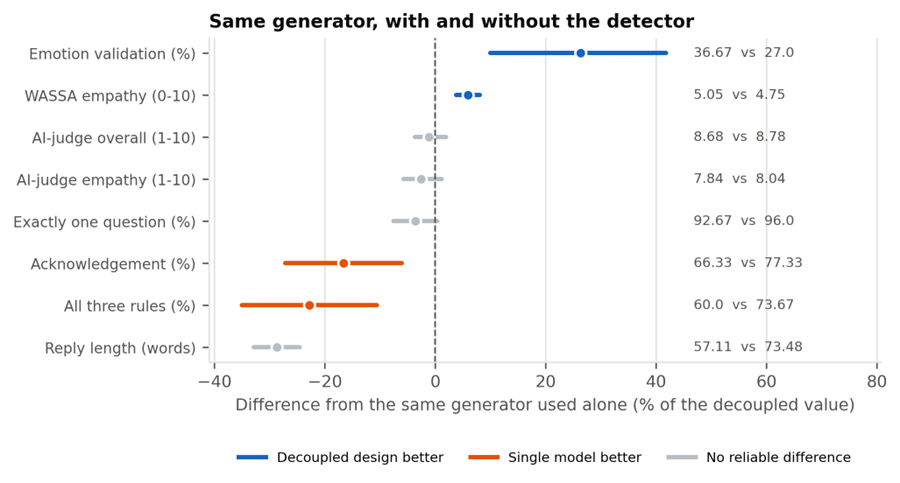
\includegraphics[width=\columnwidth]{fig_same_generator.png}}
\caption{The decoupled design against the same generator used alone, measure by measure.}
\label{fig:samegen}
\end{figure}

\subsection{Against Every Baseline}
Fig.~\ref{fig:baselines} gathers the paired comparisons. Empathy and fidelity improve reliably over every comparable design: the classifier score is at least 0.16 points higher and fidelity 8.3 to 18.3 points higher than every baseline except the largest single model (adjusted $p\leq0.013$). Against the same-size single model the judges also rate it higher on empathy (+0.70, CI +0.39 to +1.01) and overall (+0.44). Its higher rule adherence against that model is \textit{not} claimed: the raw $p$ of 0.032 becomes 0.095 after correction. The 7.6B model leads on rule adherence (+22.3 points) and the classifier (+0.71), while its judge advantages do not survive correction ($p=0.073$ and $0.109$).

\begin{figure}[htbp]
\centerline{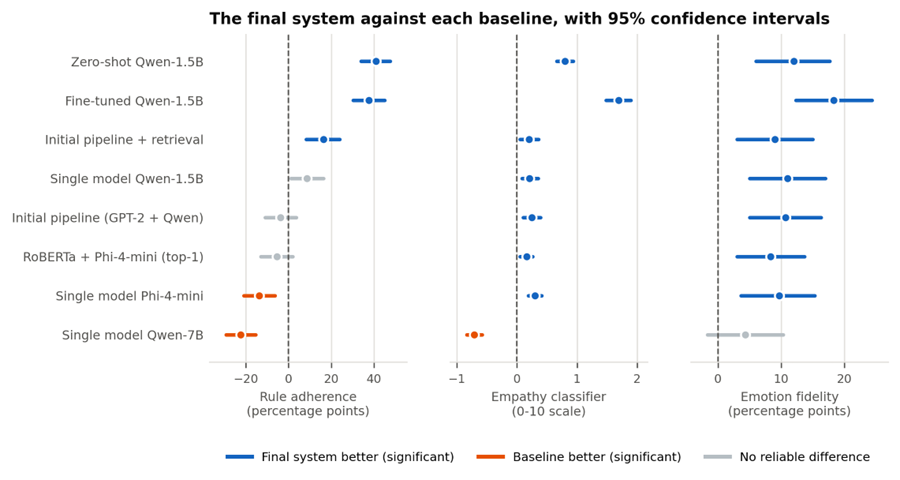
\includegraphics[width=\columnwidth]{fig_baselines.png}}
\caption{The proposed system against each baseline on three measures, with 95\% confidence intervals.}
\label{fig:baselines}
\end{figure}

\subsection{Is the Detector the Bottleneck?}
Three tests say it is not. Replies built on a wrong label are no worse in rule adherence ($p=0.40$ for the initial pipeline, $p=0.096$ for ours) or empathy (4.83 against 4.78, $p=0.72$). A more accurate detector changes nothing downstream: replacing GPT-2 with RoBERTa leaves fidelity unchanged ($p=0.91$), and substituting RoBERTa-large, 3.0 points more accurate on these conversations, changes no reply measure (all $p\geq0.60$). Most strikingly, the generator's stage-1 choice matches the gold label \textit{less} often than the detector's top prediction (42.3\% against 50.3\%, $p=0.005$), yet the two-stage system is the most emotionally faithful of all. ED gives each conversation one fine-grained label, so a reply written for \textit{terrified} when the label is \textit{afraid} counts as wrong while still answering fear. A reply needs an emotion close enough to respond to; the gain comes from how that emotion is used.

\subsection{Two Negative Results With One Cause}
Retrieval augmentation cut rule adherence from 63.7\% to 54.3\%, and to 43.7\% even with the examples filtered and an explicit one-question instruction, while the classifier (4.80 to 4.85) and fidelity (26.0\% to 27.7\%) moved within noise. Fine-tuning produced ten-word replies and 22.3\% rule adherence; an earlier configuration error that masked end-of-turn padding from the loss was found and corrected before the reported run. Both fail for one reason: only 4.3\% of the corpus's own listener replies satisfy the rules, so a method that learns behaviour from the corpus inherits a style that contradicts the specification.

\subsection{Cost and the Conversational Agent}
Over 50 messages on the same GPU, the proposed system reaches 97.5\% of the 7.6B model's overall judge score with 52\% of its parameters and 38\% less peak memory (3.40 against 5.47 GB), with no reliable difference in time (4.17 against 3.91 s, $p=0.10$; 65.7 against 65.4 ms per token). Detection and stage 1 take about 7\% of the time per reply. The 1.5B single model is lighter (2.90 GB) and 2.6 times faster, so the system is efficient relative to the model whose quality it approaches, not the smallest one.

ED conversations never change emotion, so the agent's detector window was chosen on hand-written scenarios with deliberate shifts; this is illustrative evidence, not a statistical result. Reading more helps when a message misleads alone: ``I am okay. Well, not properly'' reads as \textit{content} alone and \textit{angry} with the previous turn. A window can also be too wide: four turns was best or tied-best in three of four long scenarios, while at six a breakup scenario correct at four turns (\textit{lonely}, 61\%) flipped to \textit{guilty} at 64\%, more confident in the wrong answer than in the right one.

\section{Discussion}\label{sec:discussion}
The answer to the research question is a qualified yes. The decoupled system is parameter-efficient, resource-efficient and more emotionally faithful than single models of its own size and nearly twice its size, and it loses on rule adherence. The gains come from structure rather than generator size, since the same generator alone scores 4.75 on the classifier and 27.0\% on fidelity. The evidence is not unanimous, and the disagreement is informative: at an equal generator the judges cannot separate the two designs, while forty people reversed the AI panel's ordering against the larger model by nearly three to one. LLM judges track human preference in aggregate \cite{b32}, but on a narrow band between similar systems they did not predict what people chose. If only automatically scored quality matters and the hardware can hold a 7.6B model, that model is preferable; decoupling is the better choice when the emotional reasoning must be visible, to review a reply's tone, to show a clinician which emotion was read, or to place a safeguard before any text is written.

\textit{Limitations:} ED is English-only, crowd-sourced and single-labelled, so results may not transfer to Bangla speakers or people in genuine distress. The label set has no category for suicidal ideation: given an explicit statement of suicidal intent, the detector read \textit{afraid} (45\%) and \textit{terrified} (28\%) and the warm reply named no crisis service, so the system must not be deployed without a reviewed crisis filter and referral path \cite{b58}. Evidence rests on 300 conversations, 64 judged and 40 raters over 8 situations with weak agreement, and memory and time were measured on one GPU. Repetition remains high at 58.7\%.

\textit{Future work:} a pre-generation crisis filter comes first, followed by an ablation separating emotion selection, per-emotion guidance and cue words, which were added together. The guidance, written by the authors who are not clinicians, should be rewritten with practising counsellors; it is read at generation time, so replacing it retrains nothing. Bangla and code-mixed Bangla-English need a new 125M detector and native-speaker guidance but not a new generator, and whole conversations should be rated by mental-health professionals.

\section{Conclusion}\label{sec:conclusion}
We built an empathetic response system that separates emotion detection from response generation within the 8 GB of a consumer graphics card, and tested across 4,200 scored replies from fourteen configurations whether the separation is worthwhile. A RoBERTa-base detector feeding its top-3 emotions, cue words and emotion-specific guidance to a 4-bit Phi-4-mini produces replies that are more emotionally faithful and score higher on an independent empathy classifier than the same generator used alone, at some cost in rule adherence, and forty human raters preferred them to both a same-size and a nearly twice as large single model. Detection accuracy is not the limiting factor; how the detected emotion is used matters more. As capable open models grow smaller, how they are arranged will matter more than their size, and a sensitive application needs a design whose emotional reasoning can be examined, corrected and replaced one piece at a time.

\section*{Acknowledgment}

The authors thank their supervisor, Mr.\ Moin Mostakim, and co-supervisor, Mr.\ Sheikh Araf Noshin, of the Department of Computer Science and Engineering, BRAC University, for their guidance and continuous support, and the 40 participants who took part in the human evaluation. The system, its training and every experiment were designed, implemented and run by the authors on their own hardware, and no experimental result was produced by an AI system. In accordance with IEEE policy on AI-generated text, the authors disclose that Claude (Anthropic) was used to help draft and edit the text from the authors' results and notes, and to write parts of the analysis code that computes the reported statistics and produces the tables and figures. The authors verified all results, references and claims and take full responsibility for the content of this paper.

% The bibliography below prints its own ``References'' heading, so the template's
% separate heading and its citation instructions are kept only as comments.
% \section*{References}

% Please number citations consecutively within brackets \cite{b1}. The 
% sentence punctuation follows the bracket \cite{b2}. Refer simply to the reference 
% number, as in \cite{b3}---do not use ``Ref. \cite{b3}'' or ``reference \cite{b3}'' except at 
% the beginning of a sentence: ``Reference \cite{b3} was the first $\ldots$''

% Number footnotes separately in superscripts. Place the actual footnote at 
% the bottom of the column in which it was cited. Do not put footnotes in the 
% abstract or reference list. Use letters for table footnotes.

% Unless there are six authors or more give all authors' names; do not use 
% ``et al.''. Papers that have not been published, even if they have been 
% submitted for publication, should be cited as ``unpublished'' \cite{b4}. Papers 
% that have been accepted for publication should be cited as ``in press'' \cite{b5}. 
% Capitalize only the first word in a paper title, except for proper nouns and 
% element symbols.

% For papers published in translation journals, please give the English 
% citation first, followed by the original foreign-language citation \cite{b6}.


\begin{thebibliography}{00}
\bibitem{b1} World Health Organization, World Mental Health Report: Transforming Mental Health for All. Geneva, Switzerland: WHO, 2022. [Online]. Available: https://www.who.int/publications/i/item/9789240049338
\bibitem{b2} A. Sharma, A. S. Miner, D. C. Atkins, and T. Althoff, ``A computational approach to understanding empathy expressed in text-based mental health support,'' in Proc. 2020 Conf. Empirical Methods Natural Language Processing (EMNLP), 2020, pp. 5263--5276, doi: 10.18653/v1/2020.emnlp-main.425.
\bibitem{b3} Substance Abuse and Mental Health Services Administration, Enhancing Motivation for Change in Substance Use Disorder Treatment, Treatment Improvement Protocol (TIP) Series No. 35, SAMHSA Publication No. PEP19-02-01-003. Rockville, MD, USA: SAMHSA, 2019, ch. 3.
\bibitem{b4} Z. Lin, A. Madotto, J. Shin, P. Xu, and P. Fung, ``MoEL: Mixture of empathetic listeners,'' in Proc. 2019 Conf. Empirical Methods Natural Language Processing and 9th Int. Joint Conf. Natural Language Processing (EMNLP-IJCNLP), 2019, pp. 121--132, doi: 10.18653/v1/D19-1012.
\bibitem{b5} N. Majumder, P. Hong, S. Peng, J. Lu, D. Ghosal, A. Gelbukh, R. Mihalcea, and S. Poria, ``MIME: MIMicking emotions for empathetic response generation,'' in Proc. 2020 Conf. Empirical Methods Natural Language Processing (EMNLP), 2020, pp. 8968--8979, doi: 10.18653/v1/2020.emnlp-main.721.
\bibitem{b6} Q. Li, H. Chen, Z. Ren, P. Ren, Z. Tu, and Z. Chen, ``EmpDG: Multi-resolution interactive empathetic dialogue generation,'' in Proc. 28th Int. Conf. Computational Linguistics (COLING), 2020, pp. 4454--4466, doi: 10.18653/v1/2020.coling-main.394.
\bibitem{b7} Q. Li, P. Li, Z. Ren, P. Ren, and Z. Chen, ``Knowledge bridging for empathetic dialogue generation,'' in Proc. AAAI Conf. Artificial Intelligence, vol. 36, no. 10, 2022, pp. 10993--11001.
\bibitem{b8} S. Sabour, C. Zheng, and M. Huang, ``CEM: Commonsense-aware empathetic response generation,'' in Proc. AAAI Conf. Artificial Intelligence, vol. 36, no. 10, 2022, pp. 11229--11237.
\bibitem{b9} J. Zhou, C. Zheng, B. Wang, Z. Zhang, and M. Huang, ``CASE: Aligning coarse-to-fine cognition and affection for empathetic response generation,'' in Proc. 61st Annu. Meeting Assoc. Comput. Linguistics (ACL), vol. 1, 2023, pp. 8223--8237, doi: 10.18653/v1/2023.acl-long.457.
\bibitem{b10} Z. Yang, Z. Ren, Y. Wang, X. Zhu, Z. Chen, T. Cai, Y. Wu, Y. Su, S. Ju, and X. Liao, ``Exploiting emotion-semantic correlations for empathetic response generation,'' in Findings Assoc. Comput. Linguistics: EMNLP 2023, 2023, pp. 4826--4837, doi: 10.18653/v1/2023.findings-emnlp.320.
\bibitem{b11} Y. Qian, W.-N. Zhang, and T. Liu, ``Harnessing the power of large language models for empathetic response generation: Empirical investigations and improvements,'' in Findings Assoc. Comput. Linguistics: EMNLP 2023, 2023; arXiv:2310.05140.
\bibitem{b12} S. B. Loh and A. S. Raamkumar, ``Harnessing large language models' empathetic response generation capabilities for online mental health counselling support,'' arXiv:2310.08017, 2023.
\bibitem{b13} H. Cao, Y. Zhang, S. Feng, X. Yang, D. Wang, and Y. Zhang, ``TOOL-ED: Enhancing empathetic response generation with the tool calling capability of LLM,'' in Proc. 31st Int. Conf. Computational Linguistics (COLING), Abu Dhabi, UAE, 2025, pp. 5305--5320.
\bibitem{b14} J. Wu, X. Huang, Z. Zhu, and S. Wang, ``From traits to empathy: Personality-aware multimodal empathetic response generation,'' in Proc. 31st Int. Conf. Computational Linguistics (COLING), Abu Dhabi, UAE, 2025, pp. 8925--8938.
\bibitem{b15} Z. Li, G. Chen, R. Shao, Y. Xie, D. Jiang, and L. Nie, ``Enhancing emotional generation capability of large language models via emotional chain-of-thought,'' arXiv:2401.06836, 2024.
\bibitem{b16} S. Feng, G. Sun, N. Lubis, W. Wu, C. Zhang, and M. Gasic, ``Affect recognition in conversations using large language models,'' arXiv:2309.12881, 2023.
\bibitem{b17} T. D. Belay, I. A. Azime, A. A. Ayele, G. Sidorov, D. Klakow, P. Slusallek, O. Kolesnikova, and S. M. Yimam, ``Evaluating the capabilities of large language models for multi-label emotion understanding,'' in Proc. 31st Int. Conf. Computational Linguistics (COLING), Abu Dhabi, UAE, 2025, pp. 3523--3540.
\bibitem{b18} V. Sorin, D. Brin, Y. Barash, E. Konen, A. Charney, G. Nadkarni, and E. Klang, ``Large language models and empathy: Systematic review,'' J. Med. Internet Res., vol. 26, p. e52597, 2024, doi: 10.2196/52597.
\bibitem{b19} Z. Yang, Z. Ren, Y. Wang, S. Peng, H. Sun, X. Zhu, and X. Liao, ``Enhancing empathetic response generation by augmenting LLMs with small-scale empathetic models,'' arXiv:2402.11801, 2024.
\bibitem{b20} H. Rashkin, E. M. Smith, M. Li, and Y.-L. Boureau, ``Towards empathetic open-domain conversation models: A new benchmark and dataset,'' in Proc. 57th Annu. Meeting Assoc. Comput. Linguistics (ACL), Florence, Italy, 2019, pp. 5370--5381, doi: 10.18653/v1/P19-1534.
\bibitem{b21} Facebook Research, ``EmpatheticDialogues,'' GitHub repository (CC BY-NC 4.0 licence). [Online]. Available: https://github.com/facebookresearch/EmpatheticDialogues
\bibitem{b22} Y. Liu, W. Maier, W. Minker, and S. Ultes, ``Empathetic dialogue generation with pre-trained RoBERTa-GPT2 and external knowledge,'' in Proc. Int. Workshop Spoken Dialogue System Technology (IWSDS), 2021; arXiv:2109.03004.
\bibitem{b23} A. Welivita and P. Pu, ``A taxonomy of empathetic response intents in human social conversations,'' in Proc. 28th Int. Conf. Computational Linguistics (COLING), 2020, pp. 4886--4899, doi: 10.18653/v1/2020.coling-main.429.
\bibitem{b24} S. Wang, R. Fang, Z. He, S. Song, and Y. Li, ``Emotional support with LLM-based empathetic dialogue generation,'' arXiv:2507.12820, 2025.
\bibitem{b25} A. Rasool, M. I. Shahzad, H. Aslam, V. Chan, and M. A. Arshad, ``Emotion-aware embedding fusion in large language models (Flan-T5, Llama 2, DeepSeek-R1, and ChatGPT 4) for intelligent response generation,'' AI, vol. 6, no. 3, p. 56, 2025, doi: 10.3390/ai6030056.
\bibitem{b26} S. Poria, N. Majumder, R. Mihalcea, and E. Hovy, ``Emotion recognition in conversation: Research challenges, datasets, and recent advances,'' IEEE Access, vol. 7, pp. 100943--100953, 2019, doi: 10.1109/ACCESS.2019.2929050.
\bibitem{b27} Y. Koga, S. Kando, and Y. Miyao, ``Forecasting implicit emotions elicited in conversations,'' in Proc. Annu. Meeting Assoc. Comput. Linguistics (ACL), 2023, pp. 145--152.
\bibitem{b28} A. Paranjape, A. See, K. Kenealy, H. Li, A. Hardy, P. Qi, K. R. Sadagopan, N. M. Phu, D. Soylu, and C. D. Manning, ``Neural generation meets real people: Towards emotionally engaging mixed-initiative conversations,'' in 3rd Proc. Alexa Prize (Alexa Prize 2019), 2020; arXiv:2008.12348.
\bibitem{b29} X. Lan, Y. Cheng, L. Sheng, C. Gao, and Y. Li, ``Depression detection on social media with large language models,'' arXiv:2403.10750, 2024.
\bibitem{b30} T. Tseriotou, J. Chim, I. Tsakalidis et al., ``Overview of the CLPsych 2025 shared task: Capturing mental health dynamics from social media timelines,'' in Proc. Workshop on Computational Linguistics and Clinical Psychology, 2025, pp. 193--217.
\bibitem{b31} V. Kumar, E. Ntoutsi, P. S. Rajawat, G. Medda, and D. Reforgiato Recupero, ``Unlocking LLMs: Addressing scarce data and bias challenges in mental health,'' arXiv:2412.12981, 2024.
\bibitem{b32} L. Zheng, W.-L. Chiang, Y. Sheng et al., ``Judging LLM-as-a-judge with MT-Bench and Chatbot Arena,'' in Advances in Neural Information Processing Systems (NeurIPS), Datasets and Benchmarks Track, vol. 36, 2023; arXiv:2306.05685.
\bibitem{b33} A. Panickssery, S. R. Bowman, and S. Feng, ``LLM evaluators recognize and favor their own generations,'' in Advances in Neural Information Processing Systems (NeurIPS), vol. 37, 2024; arXiv:2404.13076.
\bibitem{b34} P. Verga, S. Hofstatter, S. Althammer, Y. Su, A. Piktus, A. Arkhangorodsky, M. Xu, N. White, and P. Lewis, ``Replacing judges with juries: Evaluating LLM generations with a panel of diverse models,'' arXiv:2404.18796, 2024.
\bibitem{b35} S. Giorgi, J. Sedoc, V. Barriere, and S. Tafreshi, ``Findings of WASSA 2024 shared task on empathy and personality detection in interactions,'' in Proc. 14th Workshop Computational Approaches to Subjectivity, Sentiment, \& Social Media Analysis (WASSA), 2024, pp. 369--379, doi: 10.18653/v1/2024.wassa-1.30.
\bibitem{b36} H. Yang, L. Huang, T. Li, N. Rusnachenko, and H. Liang, ``hyy33 at WASSA 2024 empathy and personality shared task: Using the CombinedLoss and FGM for enhancing BERT-based models in emotion and empathy prediction from conversation turns,'' in Proc. 14th Workshop Computational Approaches to Subjectivity, Sentiment, \& Social Media Analysis (WASSA), 2024, pp. 430--434, doi: 10.18653/v1/2024.wassa-1.39.
\bibitem{b37} D. Demszky, D. Movshovitz-Attias, J. Ko, A. Cowen, G. Nemade, and S. Ravi, ``GoEmotions: A dataset of fine-grained emotions,'' in Proc. 58th Annu. Meeting Assoc. Comput. Linguistics (ACL), 2020, pp. 4040--4054, doi: 10.18653/v1/2020.acl-main.372.
\bibitem{b38} J. Devlin, M.-W. Chang, K. Lee, and K. Toutanova, ``BERT: Pre-training of deep bidirectional transformers for language understanding,'' in Proc. 2019 Conf. North American Chapter Assoc. Comput. Linguistics (NAACL-HLT), 2019, pp. 4171--4186, doi: 10.18653/v1/N19-1423.
\bibitem{b39} Y. Liu, M. Ott, N. Goyal, J. Du, M. Joshi, D. Chen, O. Levy, M. Lewis, L. Zettlemoyer, and V. Stoyanov, ``RoBERTa: A robustly optimized BERT pretraining approach,'' arXiv:1907.11692, 2019.
\bibitem{b40} A. Vaswani, N. Shazeer, N. Parmar, J. Uszkoreit, L. Jones, A. N. Gomez, L. Kaiser, and I. Polosukhin, ``Attention is all you need,'' in Advances in Neural Information Processing Systems (NeurIPS), vol. 30, 2017, pp. 5998--6008.
\bibitem{b41} A. Abouelenin, A. Ashfaq, A. Atkinson et al. (Microsoft), ``Phi-4-Mini technical report: Compact yet powerful multimodal language models via Mixture-of-LoRAs,'' arXiv:2503.01743, 2025.
\bibitem{b42} T. Dettmers, A. Pagnoni, A. Holtzman, and L. Zettlemoyer, ``QLoRA: Efficient finetuning of quantized LLMs,'' in Advances in Neural Information Processing Systems (NeurIPS), vol. 36, 2023.
\bibitem{b43} A. Yang, B. Yang, B. Zhang, B. Hui et al. (Qwen Team), ``Qwen2.5 technical report,'' arXiv:2412.15115, 2024.
\bibitem{b44} Google, ``Gemma terms of use.'' [Online]. Available: https://ai.google.dev/gemma/terms
\bibitem{b45} A. Holtzman, J. Buys, L. Du, C. Fang, and Y. Choi, ``The curious case of neural text degeneration,'' in Proc. Int. Conf. Learning Representations (ICLR), 2020.
\bibitem{b46} E. J. Hu, Y. Shen, P. Wallis, Z. Allen-Zhu, Y. Li, S. Wang, L. Wang, and W. Chen, ``LoRA: Low-rank adaptation of large language models,'' in Proc. Int. Conf. Learning Representations (ICLR), 2022.
\bibitem{b47} P. Lewis, E. Perez, A. Piktus, F. Petroni, V. Karpukhin, N. Goyal, H. Kuttler, M. Lewis, W. Yih, T. Rocktaschel, S. Riedel, and D. Kiela, ``Retrieval-augmented generation for knowledge-intensive NLP tasks,'' in Advances in Neural Information Processing Systems (NeurIPS), vol. 33, 2020, pp. 9459--9474.
\bibitem{b48} N. Reimers and I. Gurevych, ``Sentence-BERT: Sentence embeddings using Siamese BERT-networks,'' in Proc. 2019 Conf. Empirical Methods Natural Language Processing and 9th Int. Joint Conf. Natural Language Processing (EMNLP-IJCNLP), 2019, pp. 3982--3992, doi: 10.18653/v1/D19-1410.
\bibitem{b49} Q. McNemar, ``Note on the sampling error of the difference between correlated proportions or percentages,'' Psychometrika, vol. 12, no. 2, pp. 153--157, 1947.
\bibitem{b50} F. Wilcoxon, ``Individual comparisons by ranking methods,'' Biometrics Bulletin, vol. 1, no. 6, pp. 80--83, 1945.
\bibitem{b51} B. Efron and R. J. Tibshirani, An Introduction to the Bootstrap. New York, NY, USA: Chapman \& Hall, 1993.
\bibitem{b52} S. Holm, ``A simple sequentially rejective multiple test procedure,'' Scandinavian J. Statistics, vol. 6, no. 2, pp. 65--70, 1979.
\bibitem{b53} A. Paszke, S. Gross, F. Massa, A. Lerer, J. Bradbury, G. Chanan et al., ``PyTorch: An imperative style, high-performance deep learning library,'' in Advances in Neural Information Processing Systems (NeurIPS), vol. 32, 2019, pp. 8024--8035.
\bibitem{b54} T. Wolf, L. Debut, V. Sanh, J. Chaumond, C. Delangue, A. Moi, P. Cistac, T. Rault, R. Louf, M. Funtowicz et al., ``Transformers: State-of-the-art natural language processing,'' in Proc. 2020 Conf. Empirical Methods Natural Language Processing: System Demonstrations, 2020, pp. 38--45, doi: 10.18653/v1/2020.emnlp-demos.6.
\bibitem{b55} P. Virtanen, R. Gommers, T. E. Oliphant et al., ``SciPy 1.0: Fundamental algorithms for scientific computing in Python,'' Nature Methods, vol. 17, pp. 261--272, 2020, doi: 10.1038/s41592-019-0686-2.
\bibitem{b56} F. Pedregosa, G. Varoquaux, A. Gramfort et al., ``Scikit-learn: Machine learning in Python,'' J. Machine Learning Research, vol. 12, pp. 2825--2830, 2011.
\bibitem{b57} NVIDIA, ``GeForce RTX 4060 Ti \& 4060 graphics cards: Specifications.'' [Online]. Available: https://www.nvidia.com/en-us/geforce/graphics-cards/40-series/rtx-4060-4060ti/
\bibitem{b58} World Health Organization and International Association for Suicide Prevention, Preventing Suicide: A Resource for Media Professionals, Update 2023. Geneva, Switzerland: WHO, 2023. [Online]. Available: https://www.who.int/publications/i/item/9789240076846
\end{thebibliography}
% Template instruction text, kept as comments:
% \vspace{12pt}
% \color{red}
% IEEE conference templates contain guidance text for composing and formatting conference papers. Please ensure that all template text is removed from your conference paper prior to submission to the conference. Failure to remove the template text from your paper may result in your paper not being published.

\end{document}
